\section{Implementation}
\subsection{Architecture}

Figure () shows the arrangement of the devices on the table. It shows a device on a stand with its back camera facing down onto the table which does all the vision calculation. There are a multiple of devices on the table which comes together to become a ad-hoc ubiquitous surface.

Figure () shows the architecture diagram of how the system works. The device on the stand does the vision calculation to locate all the devices and saves the coordinate of the device to the Firebase. As soon as the position gets updated the devices gets a notification which it checks to find its location on the table and show the part of the table at that location.

\subsection{Database Design}

Firebase saves the information in a JSON format on its database as a (key, value) pair. Figure \ref{firbase_design} shows the design I went with for my project.I decided to with a tree like structure and giving the users some control of their different sessions. The database is designed as a tree like, where the users can get all the information they need depending on their session name. 

The picture is colour coded, the yellow nodes are the ones that has multiple children. The green nodes are the ones dynamically named, Session Name is the name that the user inputs into the application at the beginning explained more in Section \nameref{cameraapp}. The background colour is the colour that the devices flashes initially, this will be explained more in Section \nameref{tableapp}. The background colour is the identifier I am using to detect the devices and querying the database. 

The \emph{numOFDevices} is the number of Devices that are in this session on the table. \emph{Zoom} is the value that image is zoomed to in the session, and position is the position of the device that is identified by that background colour.

\begin{figure}
\centering
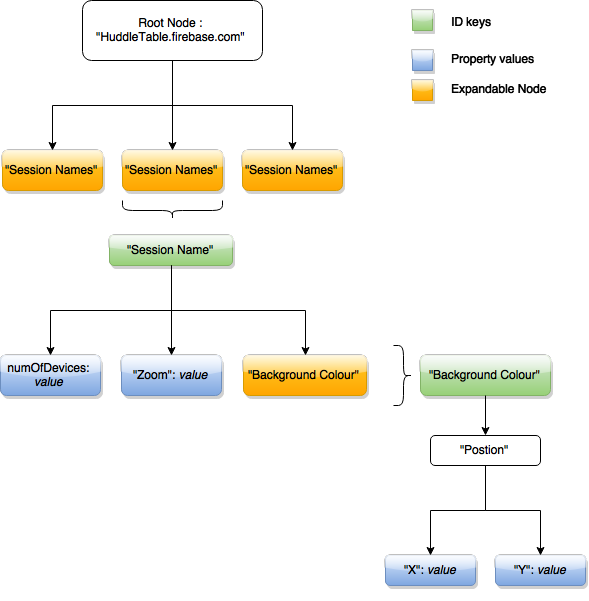
\includegraphics[scale=0.6]{firebase_design}
\caption{My Firebase database design}
\label{firebase_design}
\end{figure}


\subsection{Applications}
For this concept to come to life I had to make two different application. One has to be a replacement for the camera and the laptop in the HuddleLamp project, called the \emph{CameraApp} and the other has to be an application for all the devices on the table, called the \emph{TableApp}. This application should be able to deal with gesture control and interaction since we do not have depth sensors in this arrangement.

As ayou can see from my database design,the whole idea hinges on the "session name", therefore both application start off on a similar screen where the users can type in the session name. Figure \ref{session_screen} shows the session screen. 
\subsubsection{CameraApp} \label{cameraapp}
CameraApp was the main contribution in this Chapter. the primary aim of the CameraApp was to detect and identify devices on the table. My research in Section \ref{device_identification} shown that the most efficient method for identification in this scenario would be colour detection. To simplify the problem and to reduce the chance of overlapping I have decided to limit the colours to just the primary colours. This would mean there would be a clear distinction between the colours making it easier for the device to identify the position.
\begin{figure}[H]
    \centering
    \begin{subfigure}[b]{0.47\textwidth}
        \centering
        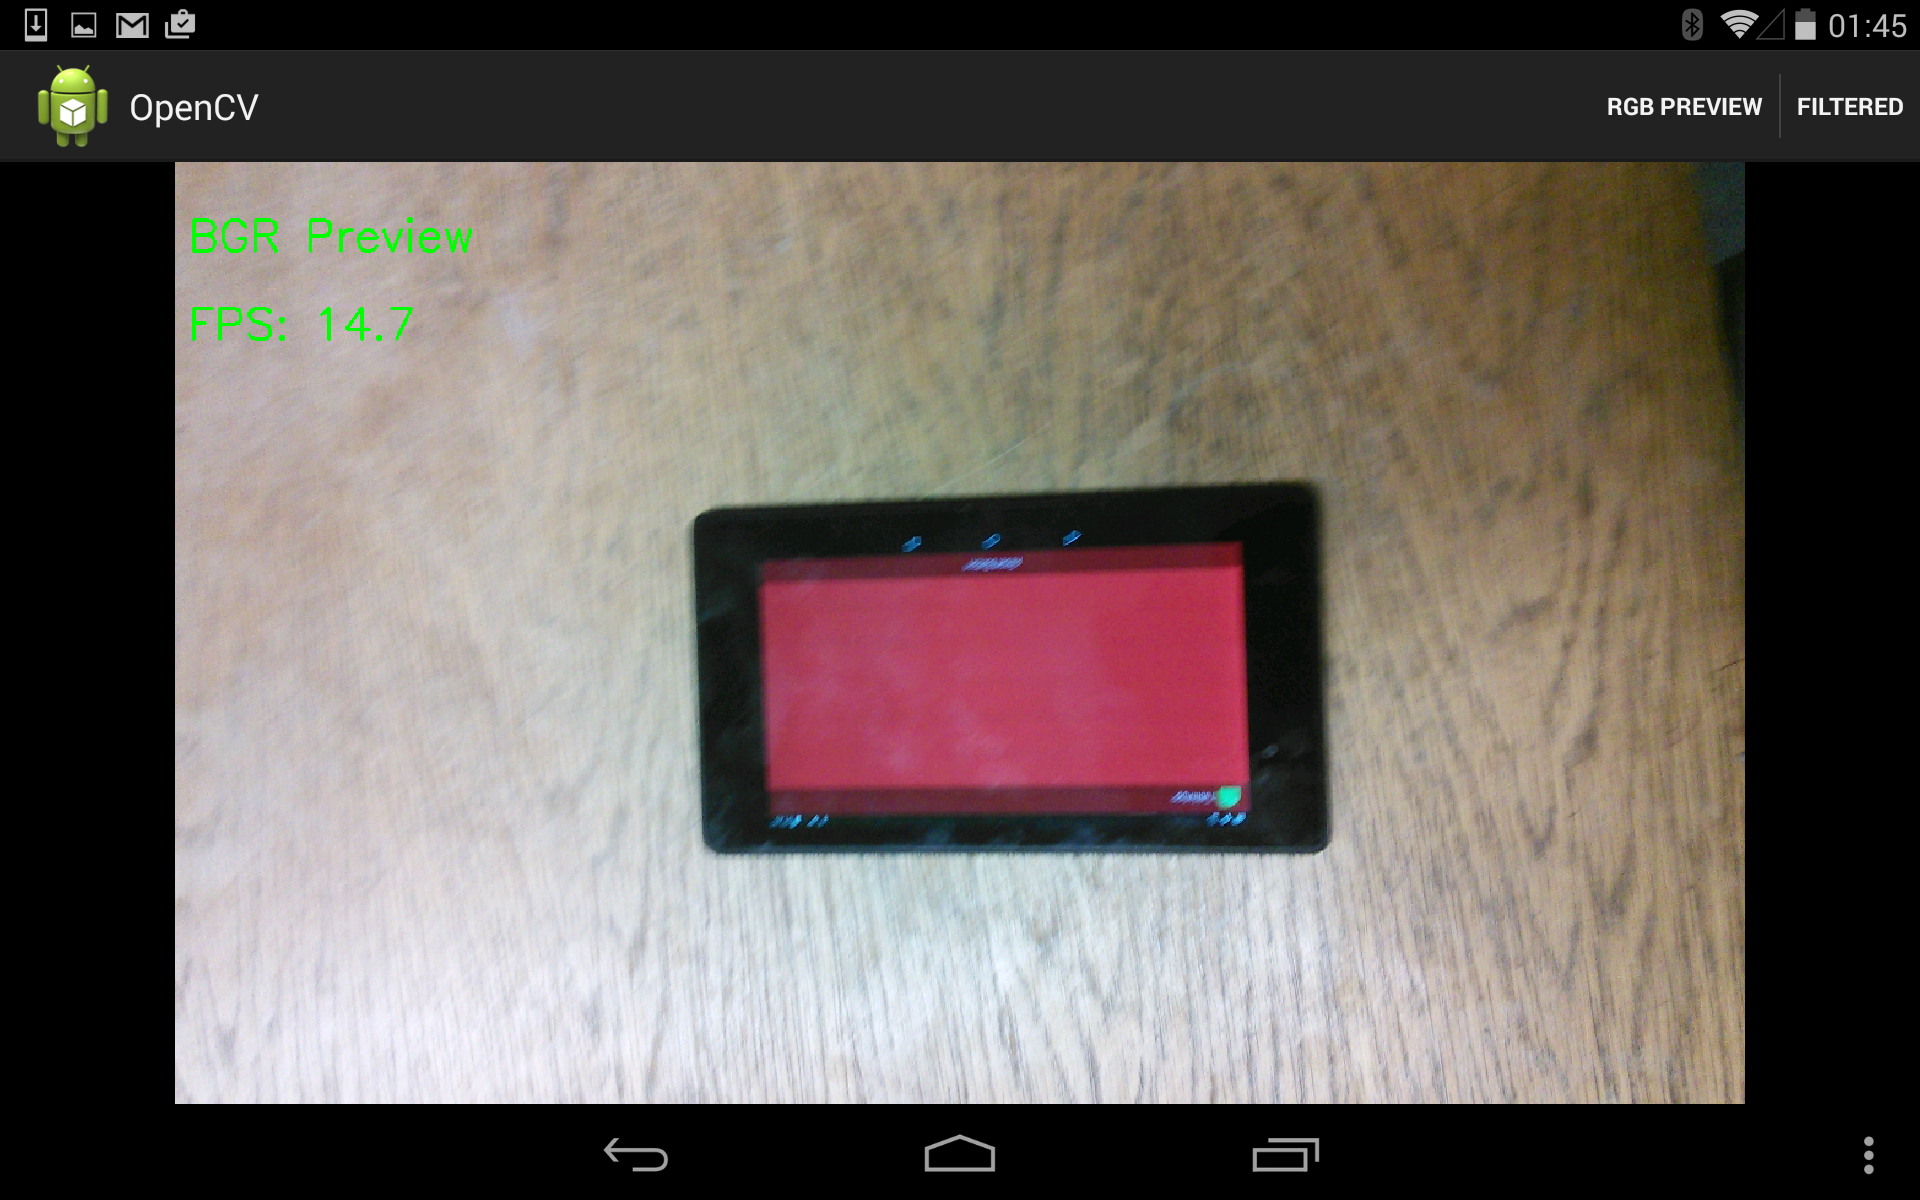
\includegraphics[width=\textwidth]{red(rgb)}
        \caption{A screen with Red area showing}
        \label{red_screen}
    \end{subfigure}
    \hfill
    \begin{subfigure}[b]{0.47\textwidth}
        \centering
        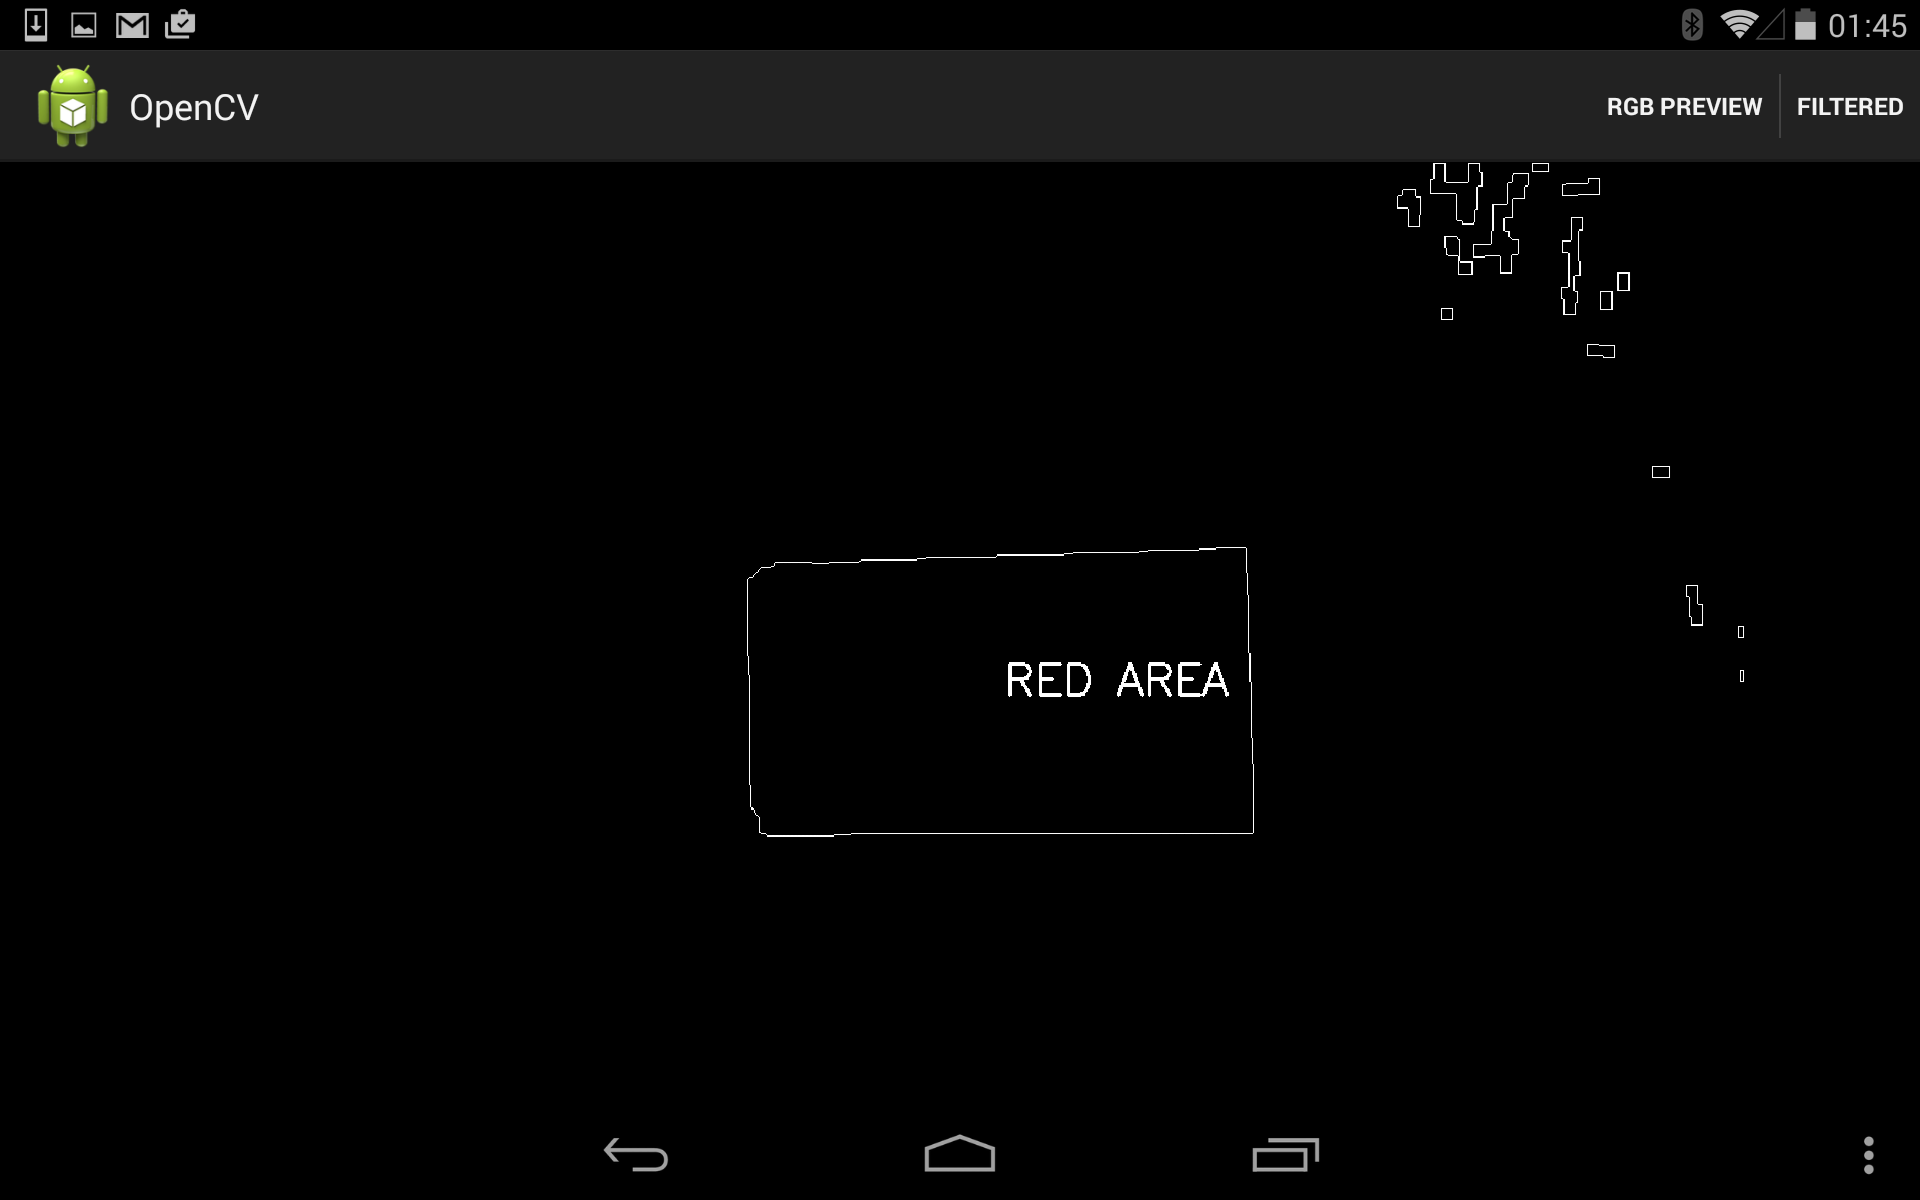
\includegraphics[width=\textwidth]{red(filtered)}
        \caption{Same frame filtered for Red}
    \end{subfigure}
    \hfill
    \caption{Screenshot of the application working for Red area}
     \label{filtered_red}
\end{figure}
As a proof of concept, and as an initial milestone I decided to try and get the CameraApp to detect large red surfaces. I had to work out the range for red colour in Hue, Saturation, Value (H, S, V) format and then filter the image for that range. Table \ref{colour_range} shows the various ranges for different colours. Figure \ref{filtered_red} shows the result of the application working for red colour.

\begin{table}[h]
\centering
\begin{tabular}{|c|c|}
\hline 
Colour & (H, S, V) Ranges\tabularnewline
\hline 
\hline 
Red & \begin{tabular}{@{}c@{}}(0, 100, 100) to (10, 255, 255) \\ \& \\ (160, 100, 100) to (179, 255, 255) \end{tabular} \tabularnewline
\hline 
Green & (40, 100, 100) to (75, 255, 255)\tabularnewline
\hline 
Blue & (100, 0, 0) to (120, 255, 255)\tabularnewline
\hline 
\end{tabular}
\caption{A table to show the Hue, Saturation and Value ranges used for the colours Red, Green and Blue}
\label{colour_range}
\end{table}

The next logical step was to get the position of those red object and store it in our data store in Firebase. This was made easier by using same key values for both application for common keys such as, position, colour name etc. By using the same Enum for the both apps for colour I was able to ensure that the colour name saved onto Firebase would be identical and Figure {} shows the final strings used as the key for other values such as position, number of Devices.

I used the view of the camera app for my coordinate system. By getting the position of the red object on the screen and translated it using the function \emph{convertToPosition()} that I wrote to work out the position. I saved it as a position object onto the data store.

The next step in the evolution of the app was to filter for other colours that the camera could see and save those position onto the data store. Figure () shows the scenario where the CameraApp was able to detect a red and green object in the image and show their respective positions. This milestone was achieved by making copies of each frame and then filtering the frames for different colour ranges. So in our case we had to make 4 copies (2 X red, blue and green) and filter them and then merge them using a weighted sum of all the arrays. OpenCV had a function called \emph{Core.addWeighted()} which was able to do this for me.
\begin{figure}[H]
    \centering
    \begin{subfigure}[b]{0.47\textwidth}
        \centering
        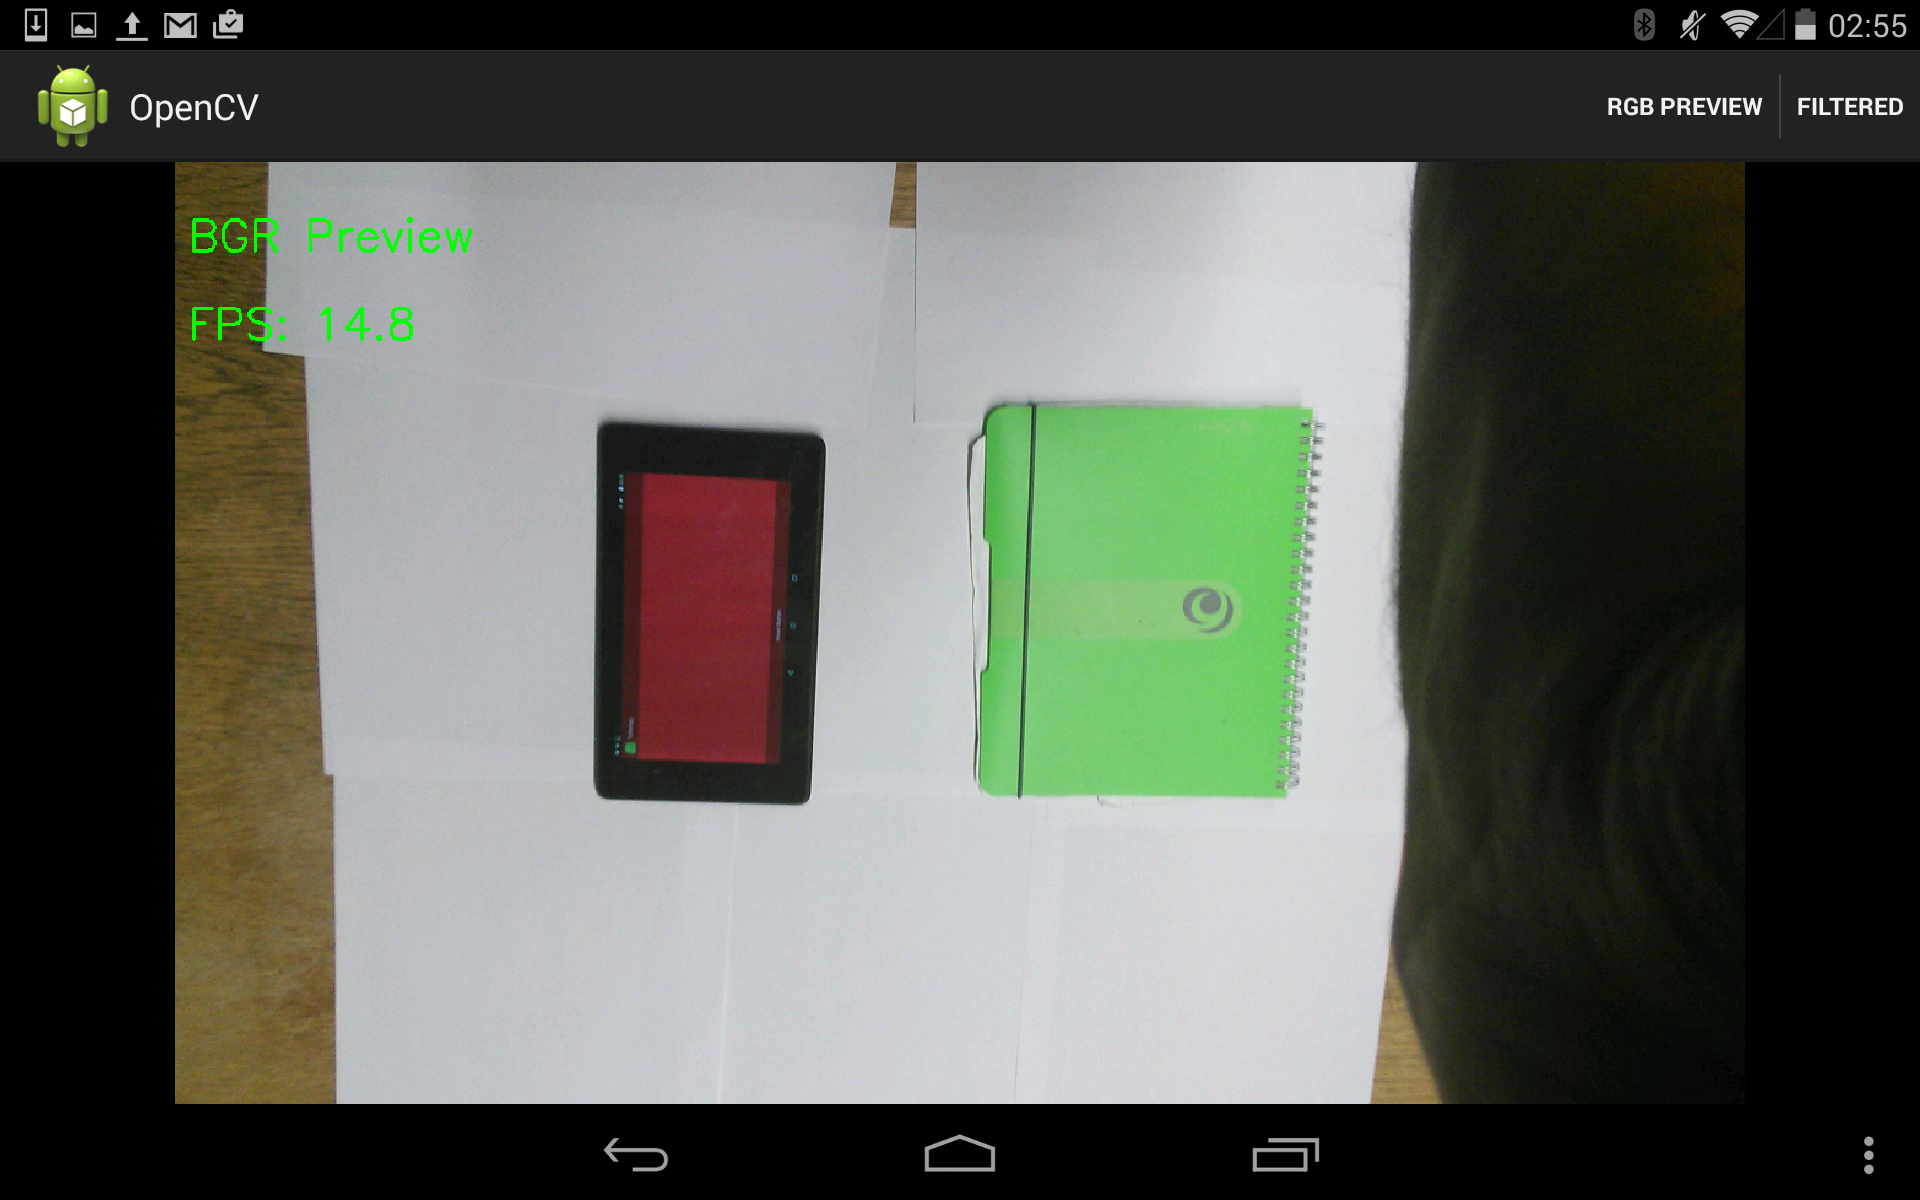
\includegraphics[width=\textwidth]{multiple(rgb)}
        \caption{A screen with Multiple colour area showing}
    \end{subfigure}
    \hfill
    \begin{subfigure}[b]{0.47\textwidth}
        \centering
        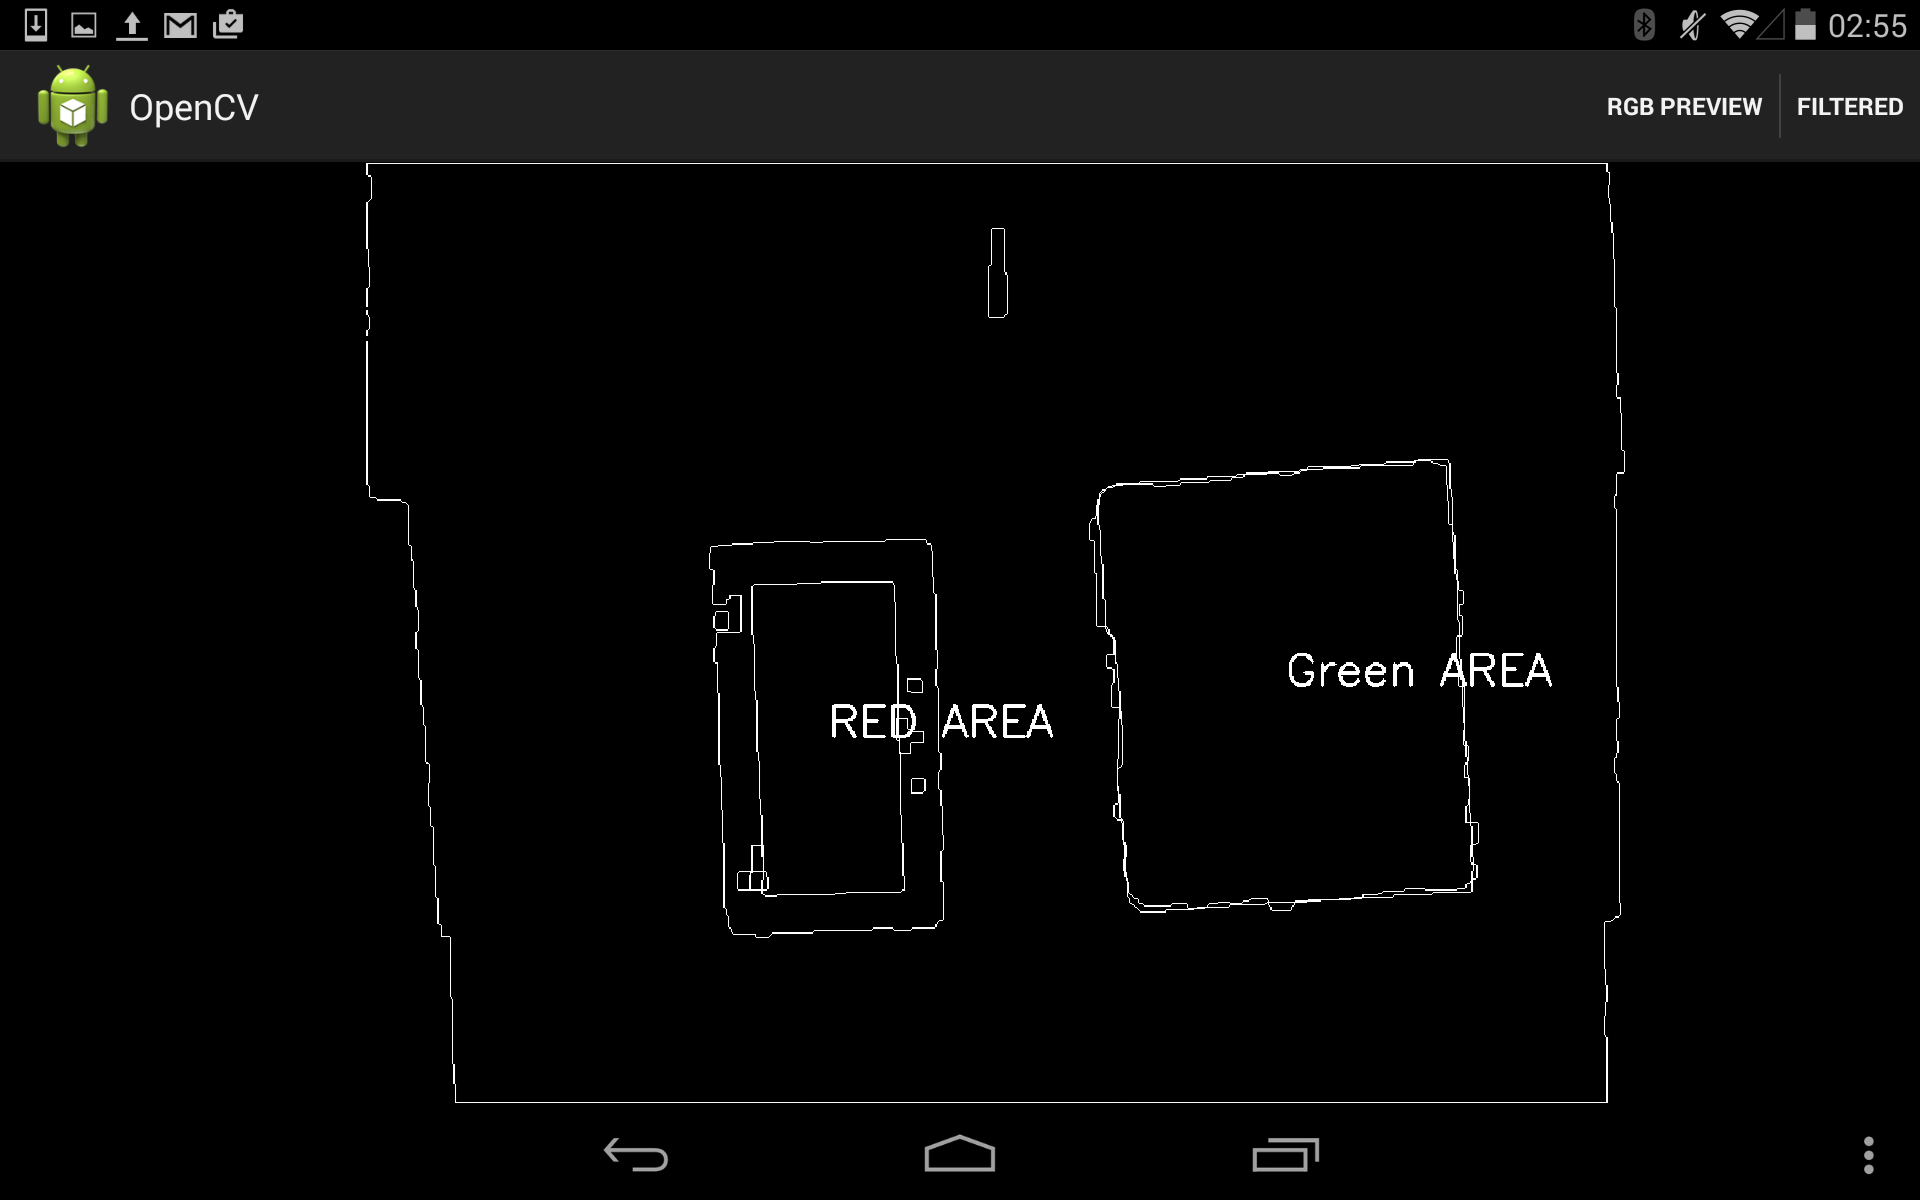
\includegraphics[width=\textwidth]{multiple(filtered)}
        \caption{Same frame filtered for Multiple colours}
    \end{subfigure}
    \hfill
    \caption{Screenshot of the application working for Multiple colour area}
     \label{filtered_red}
\end{figure}



\subsubsection{TableApp} \label{tableapp}

The second half of the application is the TableApp. This is the app that should show the content that should be shown by the interactive table and also handle the interactions. It should also help to keep track of number of devices on the table.

Whenever this application starts a new session, by hitting the \emph{submit} of the session screen, it queries the data store for number of devices in the session and then increments that number and store the number. This number is also used to determine the colour identification of this device. The colour is picked to be one of the primary colour. Figure \ref{red_screen} shows the outcome of having the screen filled with a colour.As well as updating the number of devices field of the database it initialises its own position to (0,0) depending on the background colour. If it is the first device then it initialise the number of devices to be 1 and zoom to be 1 as well.

When the device is detected by the CameraApp, it updates the position in the data store. The advantage of firebase is that when the value gets changed if you have a listener for it, it gets called automatically simulating a push notification. When the device receives the notification it removes the colour overlay and shows the image at that position.

One of the drawbacks of using Firebase as the data store was the lack of support for real numbers. Firebase only has support for Long and Integers which meant it was quite difficult to store zoom value properly. The compromise I decided was to convert the zoom value into a String and save it as a String and convert it back to a Double value when the application requires it.


